%%%%%%%%%%%%%%%%%%%% author.tex %%%%%%%%%%%%%%%%%%%%%%%%%%%%%%%%%%%
%
% sample root file for your "contribution" to a proceedings volume
%
% Use this file as a template for your own input.
%
%%%%%%%%%%%%%%%% Springer %%%%%%%%%%%%%%%%%%%%%%%%%%%%%%%%%%


\documentclass{svproc}
%
% RECOMMENDED %%%%%%%%%%%%%%%%%%%%%%%%%%%%%%%%%%%%%%%%%%%%%%%%%%%
%
\usepackage{graphicx}
\usepackage{marvosym}

%\pdfmapfile{+txfonts.map}

\usepackage[utf8]{inputenc}
\usepackage[english, russian]{babel} % Русские и английские переносы

% to typeset URLs, URIs, and DOIs
\usepackage{url}
\usepackage{hyperref}
\def\UrlFont{\rmfamily}

\def\orcidID#1{\unskip$^{[#1]}$}
\def\letter{$^{\textrm{(\Letter)}}$}

\begin{document}
\mainmatter              % start of a contribution
%
\title{ Комбинированное использование локального и глобального поиска в параллельной схеме вложенной оптимизации 
%Combining local and global search in a parallel nested optimization scheme ? 
\thanks{This study was supported by the Russian Science Foundation, project No.\,16-11-10150.}
}
%
\titlerunning{ABBR}  % abbreviated title (for running head)
%                                     also used for the TOC unless
%                                     \toctitle is used
%
\author{Konstantin Barkalov\letter\orcidID{0000-0001-5273-2471} \and Ilya Lebedev\orcidID{0000-0002-8736-0652} \and Maria Kocheganova \orcidID{0000-0002-4722-6299} \and Victor Gergel \orcidID{0000-0002-4013-2329}}
%
\authorrunning{Konstantin Barkalov et al.} % abbreviated author list (for running head)
%
%%%% list of authors for the TOC (use if author list has to be modified)
\tocauthor{Konstantin Barkalov and Ilya Lebedev, and Maria Kocheganova}
%
\institute{Lobachevsky State University of Nizhni Novgorod, Russia  \\
	\email{konstantin.barkalov@itmm.unn.ru}
}
	
\maketitle              % typeset the title of the contribution

\begin{abstract}

В статье рассматриваются задачи глобальной оптимизации и численные методы их решения. О характере зависимости целевой функции от ее параметров делается предположение, что она является многоэкстремальной лишь по некоторым из переменных, а зависимость от остальных носит локальный характер. Задачи такого типа могут возникать при идентификации неизвестных параметров математических моделей по результатам экспериментов. Предложена параллельная схема вычислений, которая учитывает данную особенность. Новая схема основана на идее nested (recursive) optimization, когда на верхнем уровне рекурсии проводится оптимизации по переменным, влияющим глобально (с помощью метода глобальной оптимизации), а на нижнем -- решение задач локальной оптимизации (с помощью локального метода). Возникающие при этом локальные подзадачи не будут оказывать влияния друг на друга, и их решение можно проводить параллельно. Проведены численные эксперименты на нескольких сотнях тестовых задач, подтверждающие эффективность предложенной схемы параллельных вычислений.


\keywords{Global optimization $\cdot$ Local optimization $\cdot$ Recursive optimization scheme $\cdot$ Parallel algorithms}
\end{abstract}

\section{Introduction}

Задачи глобальной оптимизации часто возникают в различных областях современной науки и техники. Например,  актуальными являются проблемы поиска конфигураций различных химических соединений, соответствующих минимуму энергии взаимодействия \cite{Posypkin2014}. В частности, такие задачи возникают при разработке новых лекарственных препаратов \cite{Sulimov}. Задачи глобальной оптимизации возникают и во многих других приложениях (см. обзор  \cite{Pinter2006}). 

Классическим стало применение методов глобальной оптимизации для идентификации параметров математических моделей по данным экспериментов. В задачах такого вида требуется провести поиск значений неизвестных параметров модели, при которых результаты расчетов по модели  близки к результатам, полученным экспериментально.

Число параметров, которые требуется идентифицировать подобным образом, для сложных математических моделей может составлять десятки и сотни \cite{Nurislamova2016,Akhmadullina2017}. В задачах подобной размерности регулярные методы поиска глобального решения не могут быть применены из-за чрезвычайно больших вычислительных затрат на покрытие области точками испытаний. Это остается справедливым даже в случае использования эффективных алгоритмов (например, \cite{Paulavicius2011,Evtushenko2009,Jones2009}), строящих существенно неравномерные покрытия. 

Однако в задачах идентификации моделей часто можно указать параметры, которые будут оказывать наибольшее влияние на результат. Число таких параметров, как правило, является небольшим. Остальные параметры либо оказывают незначительное влияние (в этом случае многоэкстремальность можно не учитывать), либо зависимость от второй группы параметров носит локальный характер.

Таким образом, актуальной является разработка параллельных алгоритмов минимизации существенно многомерных функций (сотни переменных), в которых учитывается разный характер зависимости целевой функции от разных групп параметров. А именно, предполагается, что целевая функция является многоэкстремальной лишь по части переменных. Остальные переменные влияют локально, т.е. по ним функция является одноэкстремальной. 
В этом случае решение задачи можно организовать по схеме nested (recursive) optimization. Решение  многоэкстремальной подзадачи, для которой требуется использовать сложные алгоритмы глобальной оптимизации, будет проводиться на верхнем уровне рекурсии.
Одноэкстремальные подзадачи (каждая из которых соответствует фиксированному набору значений первой части параметров) будут решаться на нижнем уровне. Для решения одноэкстремальных задач можно применять эффективные методы локальной оптимизации, линейного программирования или же линейной алгебры (в зависимости от характера локальных подзадач).

Текст статьи, отражающей результаты проведенного исследования, построен следующим образом. 
В Section 2 дано описание схемы вложенной оптимизации с учетом разных свойств функции на разных уровнях рекурсии. Приведен конкретный пример задачи указанного класса. Описана общая схема организации параллельных вычислений. 
Section 3 посвящен описанию параллельного алгоритма глобального поиска с использованием с использованием space-filling curves. Приведена вычислительная схема параллельного алгоритма, описаны его основные свойства.
Section 4 обсуждаются методы решения локальных подзадач в рамках схемы рекурсивной оптимизации. Дается кратное описание свойств задач поиска локального экстремума и известных методов их решения. 
Section 5 содержит результаты численных экспериментов. Здесь производится оценка масшабируемости предложенной схемы параллельных вычислений при решении серии тестовых задач.  
Section 6 concludes the paper.


\section{Nested optimization scheme}

Рассмотрим задачу оптимизации вида
\begin{eqnarray}\label{main_problem}
& f(x^\ast,y^\ast)=\min{\left\{f(x,y):x\in S, y\in D\right\}}, \nonumber \\
& S=\left\{x\in R^M: a_i\leq x_i \leq b_i, 1\leq i \leq M\right\}, \\
& D=\left\{y\in R^N: c_i\leq y_i \leq d_i, 1\leq i \leq N\right\}. \nonumber
\end{eqnarray}

Будем предполагать, что при любом фиксированном наборе значений $\overline{x}$ функция $f(\overline{x},y)$ является многоэкстремальной и удовлетворяет Lipschitz condition
\[
\left|f(\overline{x},y')-f(\overline{x},y'')\right|\leq L\left\|y'-y''\right\|,\; y',y'' \in D,\; 0<L<\infty,
\]
with the constant $L$ unknown a priori.
Одновременно с этим при любом фиксированном наборе значений $\overline{y}$  функция $f(x,\overline{y})$ является унимодальной, т.е. функция $f(x,\overline{y})$ имеет единственную точку минимума $x^*$ (зависящую, вообще говоря, от $\overline{y}$). 

Учет подобной особенности рассматриваемого класса задач может существенно снизить вычислительную сложность поиска оптимума. В самом деле, в соответствии с известной схемой рекурсивной оптимизации \cite{Carr} решение исходной задачи можно свести к задаче поиска глобального минимума функции $\varphi(y)$
\begin{equation}\label{global_problem}
\varphi(y^*) = \min_{y\in D}  \varphi (y)
\end{equation}
где 
\begin{equation}\label{local_problem}
\varphi(y) = \min_{x\in S} f(x,y).
\end{equation}
В соответствии с (\ref{global_problem}) вычисление одного значения функции $\varphi (y)$ (данный процесс будем называть search trial) подразумевает решение унимодальной задачи (\ref{local_problem}), которое может быть выполнено одним из методов локальной оптимизации. Эффективность и проработанность методов локальной оптимизации позволяет решать подзадачи (\ref{local_problem}) с точностью, значительно превышающей точность методов глобальной оптимизации. Соответственно, можно рассматривать задачу (\ref{global_problem}) как задачу глобальной оптимизации, в которой значение функции может быть вычислено с высокой точностью, но данная операция является трудоемкой. 

Конкретным примером задачи, в которой наблюдается разный характер зависимостей от разных групп параметров, может являться следующая задача аппроксимации.

Пусть в ходе эксперимента получены $m$ значений $u_j = u(t_j), 1 \leq j \leq m, $ функции $u(t)$, причем известно, что аналитическое выражение для  $u(t)$ имеет вид
\begin{equation}\label{ex_func}
u(t) = u(t,\omega,c)=\sum^{n}_{i=0}\left[c_{2i+1}\sin(\omega_it) + c_{2i+2}\cos(\omega_it)\right].	
\end{equation}
В данном выражении $c=\left(c_1,\ldots,c_{2n+2}\right)$, $\omega=\left(\omega_0,\omega_1,\ldots,\omega_n\right)$ являются неизвестными параметрами, определяющими конкретную функцию $u(t)$.

Введем меру отклонения функции $u(t,\omega,c)$ от экспериментальных данных как сумму квадратов
\[
\Delta(\omega,c)= \sum^{m}_{j=1}\left[u_j-u(t_j,\omega,c)\right]^2. 
\]
Now, following the idea of least squares fitting, it is possible to present the approximation problem as the problem of minimizing the objective function
\begin{equation}\label{ex_prob}
\Delta(\omega^*,c^*) = \min_{\omega,c} \Delta(\omega,c).	
\end{equation}
Решение $(\omega^*,c^*)$ данной задачи будет определять наилучшее приближение.

Задача (\ref{ex_prob}) может быть записана в рекурсивной форме
\begin{equation}\label{outer_prob}
\varphi(\omega^*) = \min_\omega \varphi(\omega)
\end{equation}
\begin{equation}\label{inner_prob}
\varphi(\omega) = \min_c \Delta(\omega,c).
\end{equation}
Вложенная подзадача (\ref{inner_prob}) является классической линейной задачей наименьших квадратов, и ее решение can be obtained by solving a system of linear algebraic equations regarding the unknown $c$, which can be done, e.g., by Gaussian elimination. Одновременно с этим внешняя задача (\ref{outer_prob}) будет являться, вообще говоря, многоэкстремальной и ее решение потребует значительных вычислительных ресурсов.
 
Таким образом, для решения задачи (\ref{main_problem}) в рекурсивной схеме (\ref{global_problem}), (\ref{local_problem}) можно применять параллельный алгоритм глобального поиска для решения внешних подзадач (\ref{global_problem}). При этом на каждой итерации алгоритма будет порождаться множество независимых подзадач (\ref{local_problem}), решение которых может проводиться параллельно с помощью локальных методов.
Общая схема организации вычислений с использованием нескольких процессов приведена на Fig.~\ref{MPI_tree}. 

\begin{figure}
\center{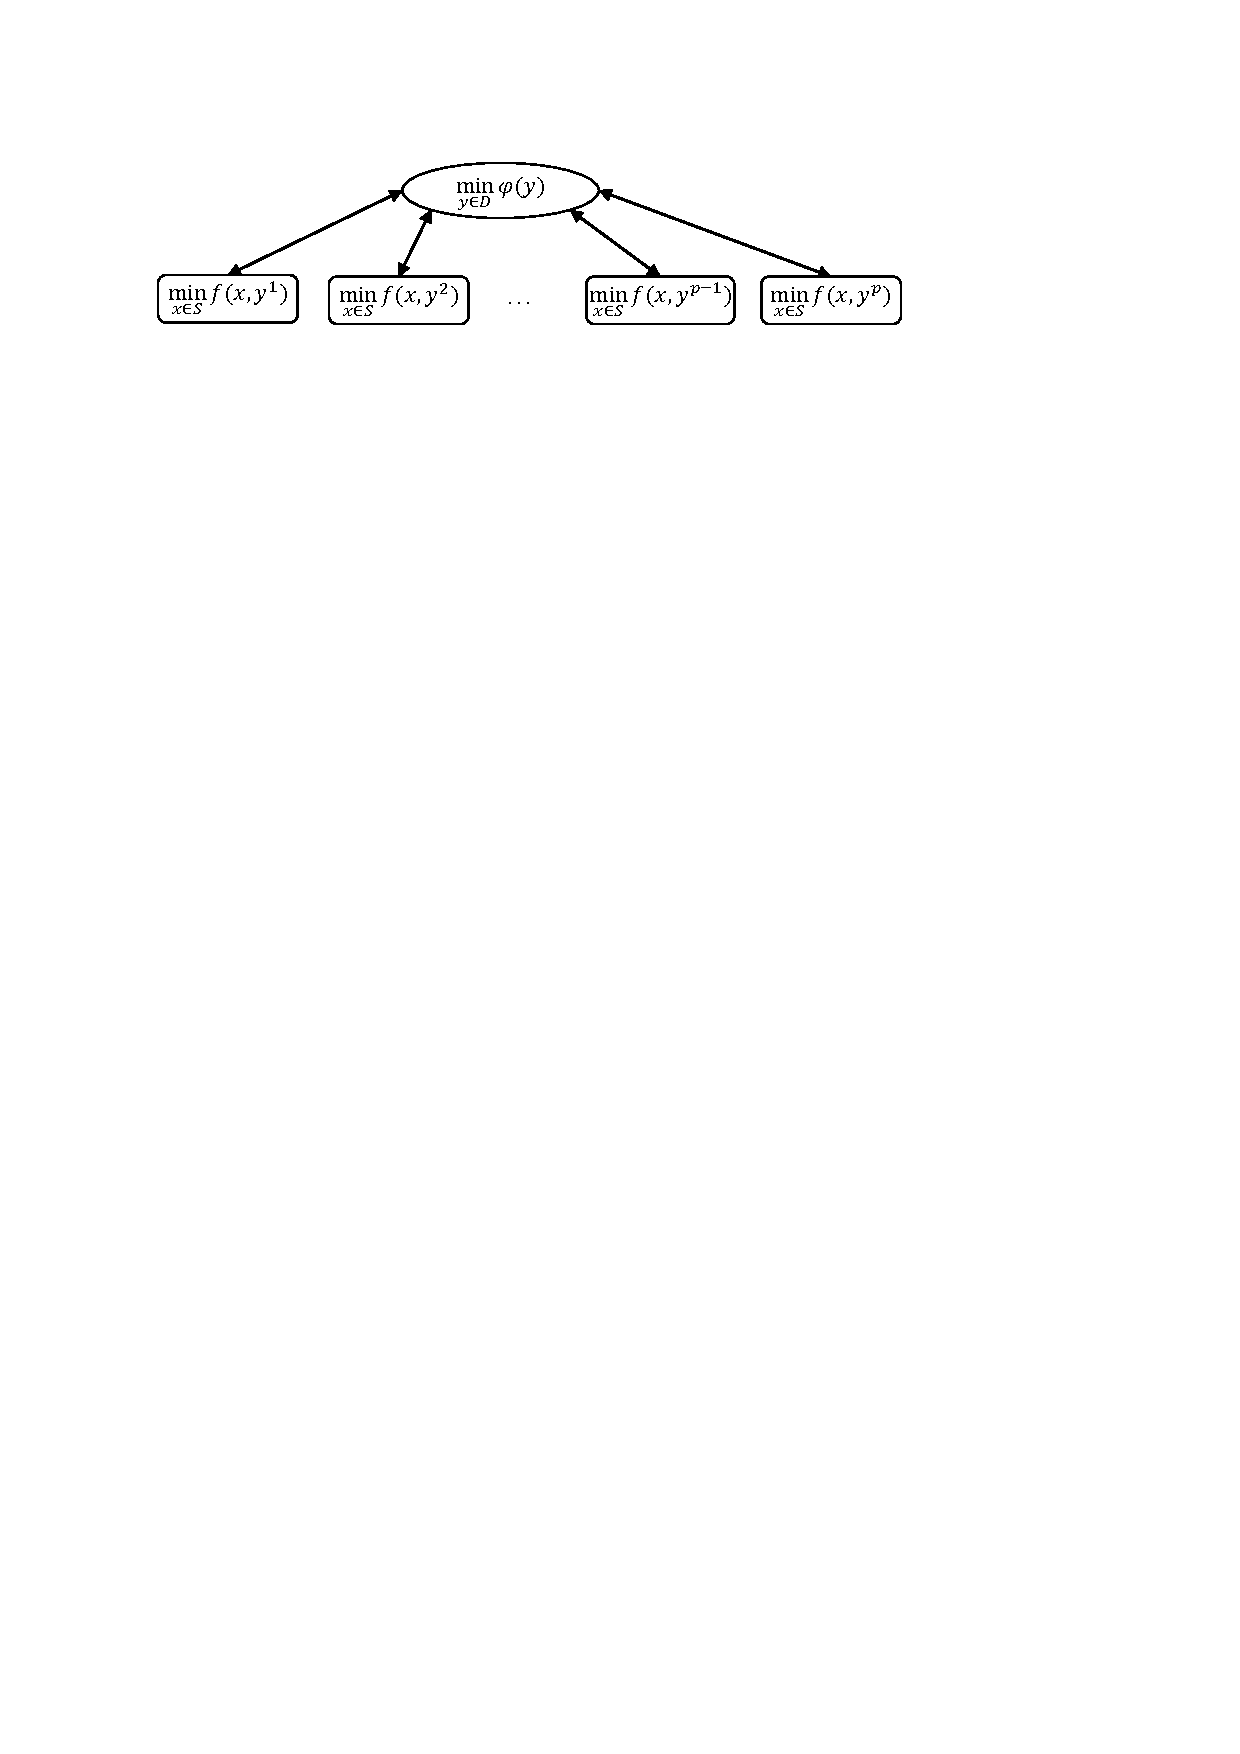
\includegraphics[width=1.0\linewidth]{MPI_Tree.pdf}}
\caption{Дерево подзадач в параллельной схеме вложенной оптимизации}
\label{MPI_tree}
\end{figure}

Процессы параллельной программы будут образовывать дерево. 
Корневой процесс будет решать задачу (\ref{global_problem}) и распределять подзадачи (\ref{local_problem}) между процессами-потомками. Каждая подзадача решается в отдельном процессе, обмен данными между процессами может быть организован с помощью MPI. Пересылки данных между процессами будут минимальные: требуется передать от корня к потомкам координаты точек $y^1, ..., y^p$ и получить обратно найденные минимальные значения 
\[
\varphi(y^1) = \min_x f(x,y^1),\; ..., \; \varphi(y^p) = \min_x f(x,y^p).
\]

Подробное обсуждение алгоритмов, используемых на разных уровнях дерева процессов, приведено в следующих разделах.  

\section{Parallel global search algorithm}

В ННГУ им. Н.И. Лобачевского был разработан \cite{Barkalov2018,Strongin2018,globalizerSystem} эффективный параллельный алгоритм глобальной оптимизации, предназначенный для решения задач вида (\ref{global_problem}) . 
Основная идея распараллеливания состоит в такой организации вычислений, при которой параллельно проводятся несколько испытаний. Этот подход характеризуется эффективностью (распараллеливается именно та часть вычислительного процесса, в котором выполняется основной объем вычислений) и общностью (применим для широкого класса алгоритмов).

В разработанном global search algorithm используется оригинальный прием снижения размерности решаемой задачи. 
Редукция размерности основана на фундаментальном факте, согласно которому $N$-мерный гиперпараллелепипед $D$ и отрезок $[0,1]$ вещественной оси являются равномощными множествами, и отрезок $[0,1]$ может быть непрерывно отображен в $D$ с помощью Peano curve $y(x)$, i.e. $D = \left\{y(x):0\leq x\leq 1\right\}$.

Используя этот факт, можно свести решение задачи минимизации многомерной функции $\varphi(y)$ к минимизации одномерной функции $\varphi(y(x))$
\begin{equation}\label{1d_problem}
\varphi(y (x^*)) = \min \left\{ \varphi (y(x)) : x\in [0,1] \right\},
\end{equation}
where the function $\varphi(y(x))$ will satisfy a uniform H{\"o}lder condition
\[
\left|\varphi(y(x'))-\varphi(y(x''))\right|\leq H\left|x'-x''\right|^{1/N}
\]
with the H{\"o}lder constant $H$ linked to the Lipschitz constant $L$ by the relation
$ H=2 L \sqrt{N+3}$ and $y(x)$ is the Peano curve from $[0,1]$ onto $D$.

The algorithms for the numerical construction of the Peano curve approximations (called \textit{evolvents})
are given in \cite{Strongin2000,Sergeyev2013}. As an illustration, two evolvents are shown in Fig.~\ref{fig_evolvent}. Figure demonstrates that the precision of the evolvent is depend on the density level $m$ used in the construction.

\begin{figure}
\center
\begin{minipage}{0.48\linewidth}
\center{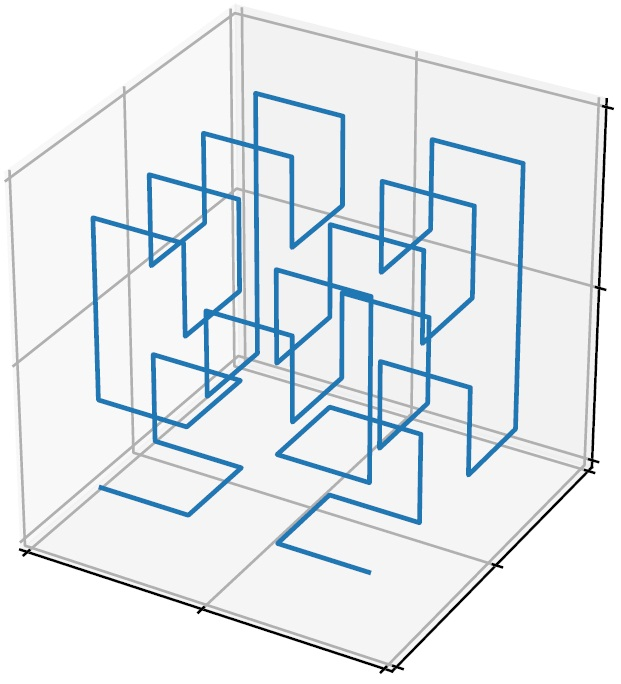
\includegraphics[width=1.0\linewidth]{fig1b.JPG} \\ (a)}
\end{minipage}
\begin{minipage}{0.48\linewidth}
\center{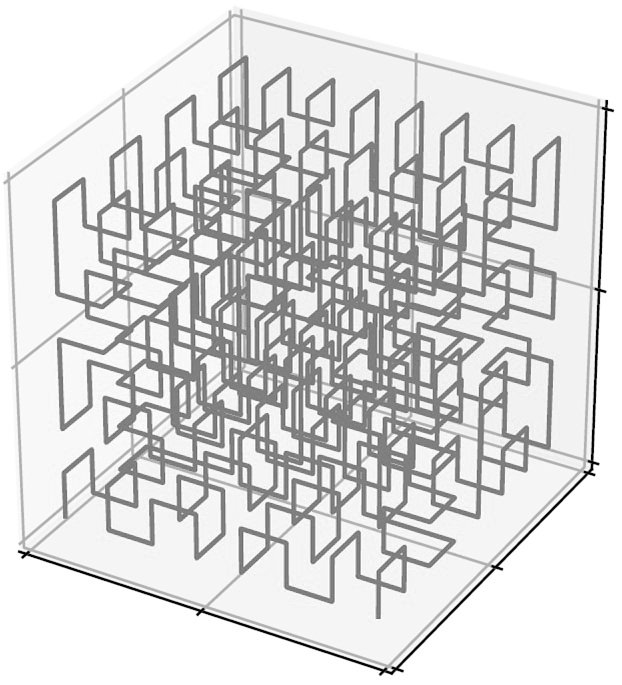
\includegraphics[width=1.0\linewidth]{fig1c.JPG} \\ (b)}
\end{minipage}
\caption{Evolvents in two dimensions with (a) $m=4$ and (b) $m=5$}
\label{fig_evolvent}
\end{figure}

Отметим, что многие известные алгоритмы глобальной оптимизации неявно основаны на идее редукции размерности и адаптации одномерных алгоритмов для решения многомерных задач \cite{Sergeyev2006,Zilinskas2008,Evtushenko2013}.

В соответствии с \cite{Strongin2000,Strongin2018} правила алгоритма глобального поиска, в котором на каждой итерации проводится параллельно $p$ испытаний, состоят в следующем.
На первой итерации метода испытания проводятся параллельно в двух граничных точках $x^1 = 0, \; x^2 = 1$, а также в $(p-2)$ произвольных внутренних точках отрезка $[0,1]$, т.е. $x^i\in(0,1),3\leq i \leq p$.

%English begin
Suppose $n\geq 1$  iterations of the method have been carried out, in which trials were performed at $k=k(n)$ points $x^i,1\leq i \leq k$. Then points $x^{k+1},\dots,x^{k+p}$  of search trials of the next iteration are determined according to the following rules.

Rule 1. Renumber the points $x^1,...,x^k$ of the preceding trials by the
lower indices in ascending order of coordinate values, i.e.
\[
0=x_1<x_2<\dots <x_{k-1} <x_k=1,
\]
and juxtapose to them the values $z_i=\varphi(y(x_i)), \; 1 \leq i \leq k$, computed at these points.

Rule 2. Compute the current lower estimates
\begin{equation}\label{Rule_Mu}
\mu = \max\left\{ \frac{\left|z_i-z_{i-1}\right|}{ \Delta_i },\; 2 \leq i \leq k  \right\},
\end{equation}
where $\Delta_i = (x_i-x_{i-1})^{1/N}$. If $\mu$ is equal to zero, then assume $\mu = 1$.

Rule 3. For each interval ($x_{i-1},x_i), \; 2 \leq i \leq k,$ compute
the \textit{characteristics} $R(i)$ :
\begin{equation}\label{Rule_R}
R(i)=\Delta_i+\frac{(z_i-z_{i-1})^2}{r^2 \mu^2\Delta_i}-2\frac{z_i+z_{i-1}}{r \mu},
\end{equation}
where $\Delta_i=(x_i-x_{i-1})^{1/N}$. The value $r > 1$ is parameter of the algorithm. An appropriate selection
of $r$ allows to consider the product $r \mu$ as an estimate
of the objective function Lipschitz constant $L$.

Rule 4. Arrange characteristics  $R(i), 2 \leq i \leq k$, in decreasing order 
\begin{equation}\label{Rule_Max}
R(t_1)\geq R(t_2)\geq \dots \geq R(t_{k}) \geq R(t_{k})
\end{equation}
and select $p$ maximum characteristics with interval numbers $t_j, 1\leq j \leq p$.

Rule 5. Carry out new trials at points $x^{k+j}\in(x_{t_j-1},x_{t_j}), \; 1\leq j\leq p$, calculated using the formulae
\begin{equation}\label{Rule_X}
x^{k+j} = \frac{x_{t_j}+x_{t_j-1}}{2} - \frac{\mathrm{sign}(z_{t_j}-z_{t_j-1})}{2r}\left[\frac{\left|z_{t_j}-z_{t_j-1}\right|}{\mu}\right]^N.
\end{equation}

The algorithm terminates if the condition $\Delta_{t_j}<\epsilon$ is satisfied at least for one number $t_j, 1 \leq j \leq p$ ; $\epsilon>0$ is the predefined accuracy.

This method of parallelization has the following justification. The characteristics of intervals (\ref{Rule_R}) used in the method can be considered as probability measures of the global minimum point location in these intervals. Inequalities (\ref{Rule_Max}) arrange intervals according to their characteristics, and trials are carried out in parallel in the first $p$ intervals with the largest probabilities.

Various modifications of this algorithm and the corresponding theory of
convergence are given in \cite{Strongin2000,Sergeyev2013,Barkalov2018,Strongin2018}.
%English end

\section{Local search algorithms}

В данном разделе рассмотрим вопросы, связанные с решением подзадачи (\ref{local_problem}), которой (при обозначении $f(x) = f(x,\overline{y})$ для фиксированного значения $\overline{y} \in D$) соответствует задача на локальный экстремум

\begin{equation} \label{lp}
f(x) \rightarrow \min, x\in S. 
\end{equation}

К настоящему времени разработано огромное количество разнообразных методов локальной оптимизации для задач вида (\ref{lp}). К их числу относятся, например, градиентные методы, ньютоновские и квазиньютоновские методы, методы сопряженных направлений. Большинство из них используют принцип локального спуска, когда метод последовательно на каждом шаге переходит к точкам с меньшими значениями целевой функции. Почти все эти методы могут быть представлены в виде итерационного соотношения
\[
x^{k+1} = x^k + s^k d^k,
\]
где $x^k$ -- точки основных испытаний, состоящих в вычислении набора тех или иных локальных характеристик целевой функции $I^k=I(x^k)$ в точке $x^k$, $d^k$ -- направления смещения из точек $x^k$, вычисляемые по результатам основных испытаний, а $s^k$ -- коэффициенты, определяющие величины смещений вдоль выбранных направлений.

Для определения величин смещений $s^k$ вдоль направлений $d^k$ методы могут выполнять вспомогательные (рабочие) шаги. Это приводит к дополнительным измерениям локальных характеристик целевой функции вдоль направления $d^k$. Переходы от точек $x^k$ к точкам $x^{k+1}$ выполняются таким образом, чтобы обеспечить существенное убывание значений функции $f^k = f( x^k )$ в результате шага.

В набор вычисляемых локальных характеристик $I^k=I(x^k)$ могут входить: значение функции $f^k = f( x^k )$, вектор градиента $\nabla f^k = \nabla f(x^k)$, матрица вторых производных (гессиан) $\Gamma_k=\Gamma^f(x^k)$. Какой именно набор характеристик измеряется -- зависит как от свойств решаемой задачи, так и от выбранного метода оптимизации.

В задачах локальной оптимизации, возникающих в приложениях, априорная информация о функциях бывает достаточно ограниченной. Например, может предполагаться лишь локальный характер зависимости функции от параметров, тогда как значения градиента (а, тем более, гессиана) являются неизвестными. В этом случае применяются методы прямого поиска, которые не используют каких-либо предположений о гладкости минимизируемой функции. При поиске минимума эти методы измеряют только значения функции. Правила размещения точек итераций в них основываются на некоторых эвристических логических схемах. 

Одними из популярных методов прямого поиска являются Hooke--Jeeves method \cite{HookJeeves} and Nelder--Mead method \cite{NelderMead}. Несмотря на кажущуюся простоту и теоретическую необоснованность методов прямого поиска, они хорошо зарекомендовали себя в реальных расчетах. Это можно объяснить следующим образом. Многие методы гладкой оптимизации чрезвычайно чувствительны к наличию вычислительных ошибок в значениях функций, превращающих теоретически гладкую функцию в фактически негладкую. За счет этого в реальных расчетах они зачастую утрачивают те положительные свойства, которые для них обещает теория. Использование методов прямого поиска позволяет в этих условиях добиться лучших результатов.

\section{Numerical experiments}

Схема параллельных вычислений, описанная в предыдущих разделах, была реализована в программной системе Globalizer, разрабатываемой в ННГУ им. Н.И. Лобачевского \cite{globalizerSystem,Sysoyev2017}.  
Вычислительные эксперименты проводились на  Lomonosov supercomputer (Lomonosov Moscow State University); узел суперкомпьютера располагает two quad-core processors Intel Xeon X5570 2.93GHz and 12 Gb RAM. При сборке системы Globalizer для запуска на Lomonosov использовался  GCC 5.5.0 compiler and Intel MPI 2017.

С целью имитации прикладных задач, в которых можно выделить параметры, влияющие локально, при проведении экспериментов использовались тестовые функции вида 
\begin{equation}\label{test_problem}
f(x,y) = G(y)+R(x),
\end{equation}
где $G(y)$ -- многоэкстремальная функция размерности $N=2$, а $R(x)$ -- унимодальная функция размертности $N \gg 2$.
В качестве многоэкстрмальной части задачи рассматривались функции 
\begin{eqnarray} \nonumber \label{vagris}
G(y)= -&\left\{\left(\sum^{7}_{i=1}\sum^{7}_{j=1}A_{ij}g_{ij}(y)+B_{ij}h_{ij}(y)\right)^2+\right. \\
&\left.\left(\sum^{7}_{i=1}\sum^{7}_{j=1}C_{ij}g_{ij}(y)+D_{ij}h_{ij}(y)\right)^2\right\}^{1/2},\\ \nonumber
\end{eqnarray}
where
\begin{eqnarray} \nonumber
& y=(y_1,y_2)\in R^2, 0 \leq y_1,y_2 \leq 1, \\ \nonumber
& g_{ij}(y)=\sin(i\pi y_1)\sin(j\pi y_2),  \\ \nonumber
& h_{ij}(y)=\cos(i\pi y_1)\cos(j\pi y_2), \nonumber 
\end{eqnarray}
and coefficients $A_{ij}, B_{ij}, C_{ij}, D_{ij}$  are taken uniformly in the interval $[-1,1]$.
Данный класс функций часто используется для тестирования алгоритмов глобальной оптимизации.  
В качестве локальной части задачи использовалась модифицированная функция Розенброка 
\[
R(x)= \sum_{i=1}^{N-1}{\left[(1-x_i)^2+100(x_{i+1}-x_i^2)^2\right]}, -2 \leq x_i \leq 2 , 1\leq i\leq N,
\]
в которой точка экстремума смещалась случайным образом в области поиска с помощью линейного преобразования координат.

В качестве примера на Fig.~\ref{fig_level}(a),(b) приведены линии уровня одной пары функций $G(y)$ и $R(x)$. Данные функции являются сложными для соответствующих методов глобальной и локальной оптимизации, т.к. функции $G(y)$ являются существенно многоэкстремальными, а функции $R(x)$ обладают ярко выраженной овражной структурой.

\begin{figure}
\center
\begin{minipage}{0.48\linewidth}
\center{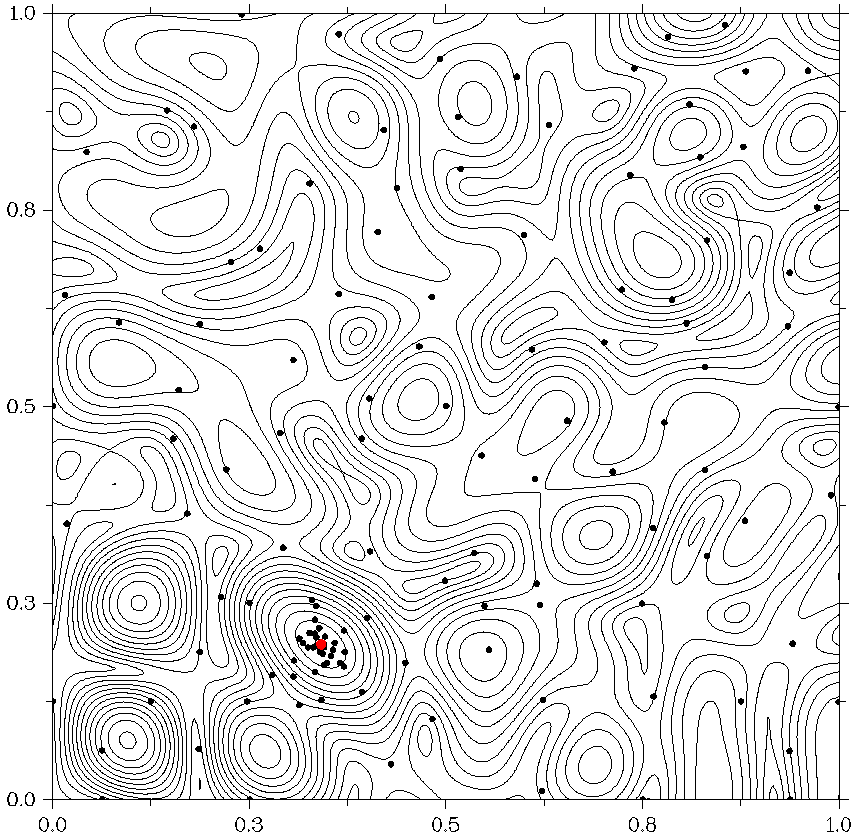
\includegraphics[width=1.0\linewidth]{grishagin.png} \\ (a)}
\end{minipage}
\begin{minipage}{0.48\linewidth}
\center{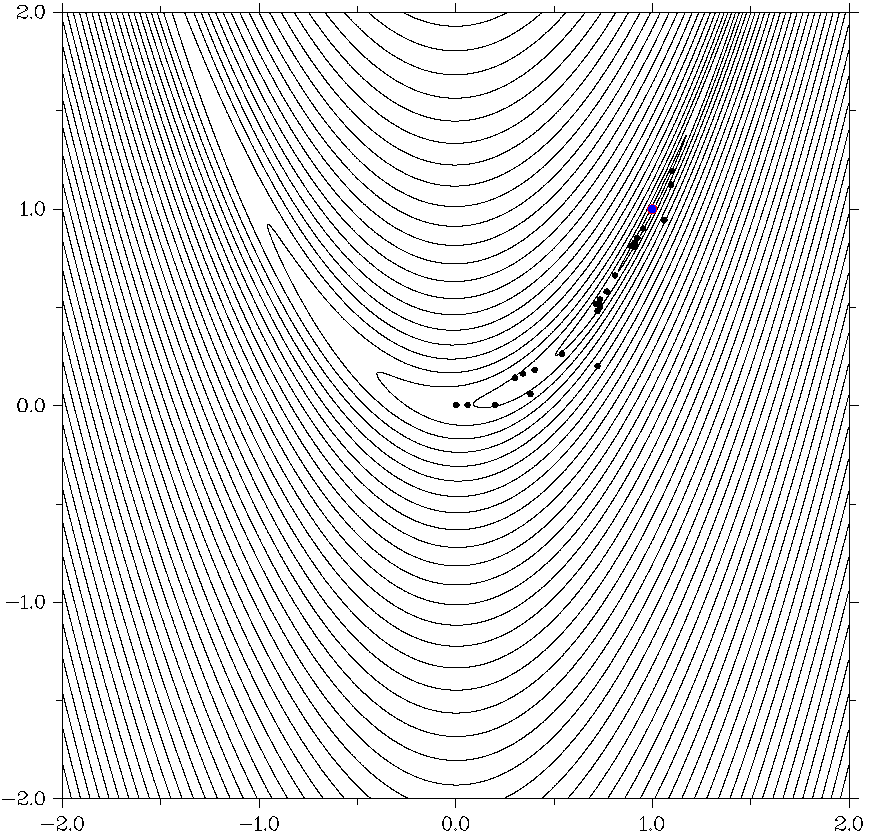
\includegraphics[width=1.0\linewidth]{rosenbrock.png} \\ (b)}
\end{minipage}
\caption{Линии уровня функций (a) $G(y)$ и (b) $R(x)$}
\label{fig_level}
\end{figure}

На Fig.~\ref{fig_level} отмечены также точки испытаний, выполненных global search algorithm and Hooke--Jeeves method при решении соответствующих задач. Расположение точек испытаний наглядно иллюстрирует как многоэкстремальность функции $G(y)$ (точки испытаний образуют неравномерную сетку в области поиска), так и овражность функции $R(x)$ (точки испытаний вытянуты вдоль дна оврага).

Задача считалась решенной, если в процессе минимизации функции $G(y)$ алгоритм глобального поиска сгенерировал точку очередного испытания $y^k$ в $\epsilon$-окрестности глобального минимума $y^*$, т.е. $\left\|y^* - y^k\right\|\leq\epsilon$, где $\epsilon = 10^{-2}$. 
При этом точность поиска минимума при минимизации унимодальной функции $R(x)$ выбиралась в 1000 раз меньше, т.е. $\delta = 10^{-5}$.
В алгоритме глобального поиска использовался параметр $r=4.5$ из (\ref{Rule_R}) и параметр построения развертки $m=10$; использованный локальный метод не имел дополнительных параметров.

В первой серии экспериментов были решены 100 задач вида (\ref{test_problem}), в которых размерность локальных подзадач равнялась $N=50$. Задачи решались на 1, 4 и 8 узлах кластера на которых было задействовано от 2 до 32 MPI-процессов. В соответствии со схемой распараллеливания, представленной на Fig.~\ref{MPI_tree}, решение задачи глобальной оптимизации на верхнем уровне рекурсии проводится в одном (главном) процессе, который инициирует параллельное решение локальных задач задач нижнего уровня (от 1 до 31 задачи соответственно). Таким образом, минимально возможное число задействованных процессов равно 2: по одному на каждом уровне рекурсии.

В table \ref{tab1} отражено среднее число итераций $K_{av}$, выполненных алгоритмом глобального поиска при минимизации функции $G(y)$, среднее время $T_{av}$ решения задачи в целом, а также ускорение по времени $S$  в зависимости от числа $p$ используемых MPI-процессов. 

\begin{table}
\centering
\caption{Результаты решения серии задач размерности $N=52$}\label{tab1}
\begin{tabular}{cccc}
\hline\noalign{\smallskip}
 $\;\;\;p\;\;\;$  &  $\;\;\;K_{av}\;\;\;$ &  $\;\;\;T_{av}\;\;\;$ & $\;\;\;S\;\;\;$ \\
\noalign{\smallskip}\hline\noalign{\smallskip}
 2  & 349.4  & 9.14 & ---  \\
 16 & 25.6   & 0.70 & 13.2 \\
 32 & 12.9   & 0.37 & 24.6 \\
\noalign{\smallskip}\hline
\end{tabular}
\end{table}


Во второй серии экспериментов были решены 10 задач вида (\ref{test_problem}), в которых размерность локальных подзадач равнялась $N=100$. Параметр запуска аналогичны предыдущей серии экспериментов. Результаты решения приведены в table \ref{tab2}.

\begin{table}
\centering
\caption{Результаты решения серии задач размерности $N=102$}\label{tab2}
\begin{tabular}{cccc}
\hline\noalign{\smallskip}
 $\;\;\;p\;\;\;$  &  $\;\;\;K_{av}\;\;\;$ &  $\;\;\;T_{av}\;\;\;$ & $\;\;\;S\;\;\;$ \\
\noalign{\smallskip}\hline\noalign{\smallskip}
 2  & 299.1  & 41.19 & ---  \\
 16 & 22.0   & 2.92 & 14.1 \\
 32 & 11.7   & 1.50 & 27.4 \\
\noalign{\smallskip}\hline
\end{tabular}
\end{table}


\section{Conclusion}

Результаты проведенных экспериментов на серии задач оптимизации, в которых можно выделить многоэкстремальную и унимодальную части задачи, показывают, что предложенная в работе схема организации параллельных вычислений обладает хорошим потенциалом параллелизма. 
В частности, при решении серии из 100 задач с общим числом переменных 52 (из которых две переменных оказывали глобальное влияние на целевую функцию, а пятьдесят влияли локально) получено ускорение 24.6 при использовании 32 процессов. 
В случае решения задач с более сложными локальными подзадачами (с числом локальных переменных $N=100$) ускорение увеличивается вплоть до 27.4 при использовании 32 процессов.

Разработанная схема параллельных вычислений может применяться при идентификации сложных математических моделей, которые характеризуются большим числом (десятки и сотни) неизвестных параметров.

%
% ---- Bibliography ----
%
\bibliographystyle{spmpsci}
\bibliography{bibliography}{}

\end{document}
